\capitulocapa[48]{images/cap-1.png}{O que realmente é estado?}
\label{chap:o-que-e-estado}

\refstepcounter{section}
\addcontentsline{toc}{section}{\protect\numberline{\thesection}Uma alteração de cinco minutos}
\sectionmark{Uma alteração de cinco minutos}

\begin{center}
  \makebox[\textwidth][c]{%
    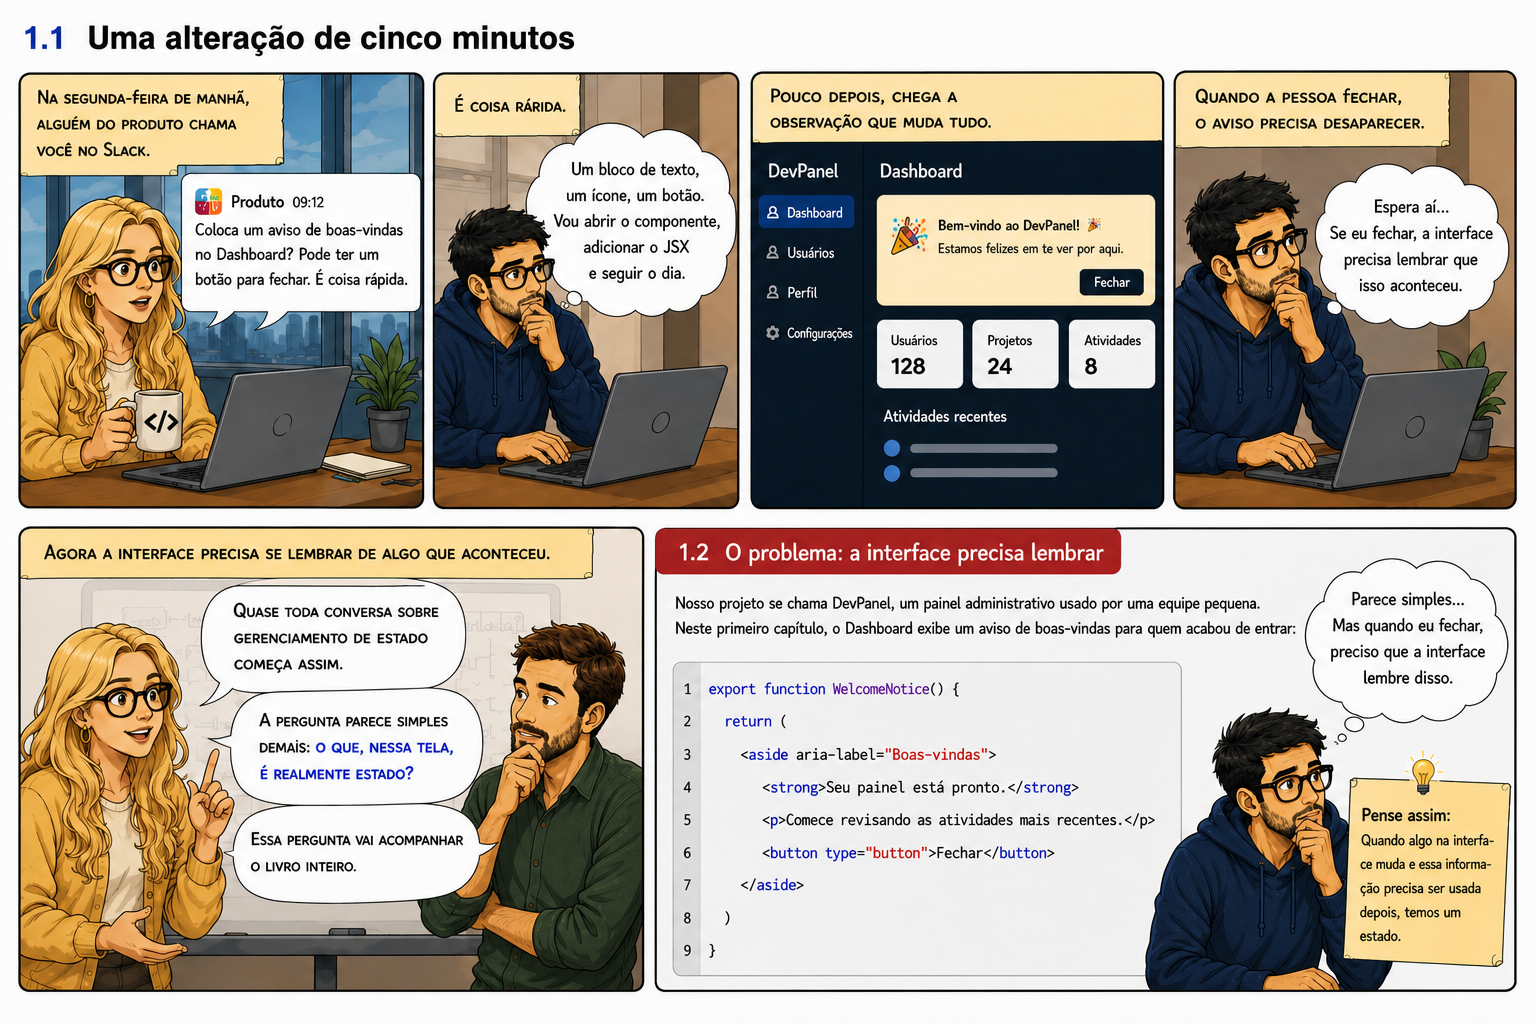
\includegraphics[width=1.16\textwidth]{images/1-1-alteracao-5-minutos-corrected.png}%
  }
\end{center}

Quase toda conversa sobre gerenciamento de estado começa assim. Não começa com
uma biblioteca. Começa com uma tela que precisa lembrar de uma escolha, reagir a
uma resposta ou representar uma etapa do trabalho.

É tentador pular direto para o código. Antes disso, vale fazer uma pergunta que
parece simples demais: \emph{o que, nessa tela, é realmente estado?}

Essa pergunta vai acompanhar o livro inteiro. Quando a resposta está errada,
nenhuma biblioteca conserta a arquitetura. Quando está certa, muitas telas nem
precisam de uma biblioteca.

\refstepcounter{section}
\addcontentsline{toc}{section}{\protect\numberline{\thesection}O problema: a interface precisa lembrar}
\sectionmark{O problema: a interface precisa lembrar}

Nosso projeto se chama DevPanel, um painel administrativo usado por uma equipe
pequena. Neste primeiro capítulo, o Dashboard exibe um aviso de boas-vindas para
quem acabou de entrar:

\begin{lstlisting}[caption={O aviso ainda não possui comportamento.}]
export function WelcomeNotice() {
  return (
    <aside aria-label="Boas-vindas">
      <strong>Seu painel está pronto.</strong>
      <p>Comece revisando as atividades mais recentes.</p>
      <button type="button">Fechar</button>
    </aside>
  )
}
\end{lstlisting}

O botão existe, mas não faz nada. Para o aviso desaparecer, o componente precisa
representar duas situações possíveis:

\begin{itemize}
  \item o aviso está visível;
  \item o aviso foi dispensado.
\end{itemize}

Essas situações não são apenas detalhes visuais. Elas dependem de uma ação que
aconteceu antes. Depois do clique, a próxima renderização precisa ser diferente
da anterior. É nesse momento que surge o estado.

\imagemcapitulo
  {ch01-diagrama-interface-estado}
  {O clique altera o estado e produz uma nova fotografia do Dashboard.}
  {interface-estado}

Uma forma prática de pensar é imaginar cada renderização como uma fotografia da
interface. O código descreve como a fotografia deve parecer para os dados
atuais. Quando uma interação altera esses dados, o React produz outra
fotografia.

Estado é a informação que precisa permanecer entre essas fotografias e cuja
mudança pode alterar o que o componente apresenta.

\section{Como normalmente resolvemos}

Quando alguém está com pressa, uma primeira tentativa comum é alterar o elemento
diretamente:

\begin{lstlisting}[caption={Uma solução que contorna o React.}]
function closeNotice() {
  document.querySelector('[aria-label="Boas-vindas"]')?.remove()
}
\end{lstlisting}

Visualmente, funciona. O elemento desaparece. O problema é que o React não sabe
que essa mudança aconteceu. Para ele, o componente continua descrevendo um
aviso que deveria existir.

Se o componente renderizar novamente por outro motivo, o aviso pode voltar. Um
teste fica dependente da estrutura do HTML. Outro componente não consegue
entender a situação atual sem consultar o DOM. Criamos duas versões da verdade:
o que o React descreve e o que foi modificado manualmente no navegador.

Outra tentativa é declarar uma variável comum:

\begin{lstlisting}[caption={A variável muda, mas a interface não reage.}]
let isNoticeVisible = true

function closeNotice() {
  isNoticeVisible = false
}
\end{lstlisting}

A variável recebe o novo valor, mas isso não pede uma nova renderização. Além
disso, ela é recriada quando pertence ao corpo do componente. Para o React,
uma variável comum não é memória reativa.

Essas tentativas revelam as duas propriedades que procuramos:

\begin{enumerate}
  \item o valor deve sobreviver de uma renderização para a próxima;
  \item alterar o valor deve solicitar uma nova renderização.
\end{enumerate}

\section{Nem toda informação é estado}

Antes de adicionar um hook, vamos classificar os valores da tela. Suponha que o
aviso também mostre o nome da pessoa e uma mensagem diferente conforme o horário:

\begin{lstlisting}
const productName = 'DevPanel'
const firstName = user.fullName.split(' ')[0]
const greeting = `${getGreeting()}, ${firstName}`
\end{lstlisting}

Os três valores aparecem na interface, mas isso não significa que os três devam
ser estados.

\subsection{Constante}

\codigo{productName} não muda durante a execução. É uma configuração conhecida.
Transformá-la em estado criaria uma operação de atualização que nunca usamos.

\subsection{Valor recebido}

Os dados do usuário podem ter vindo das propriedades. Para o componente do
aviso, eles já são uma entrada. Não precisamos copiar esse objeto para outro
estado apenas para lê-lo.

\subsection{Valor derivado}

\codigo{firstName} é calculado a partir de \codigo{user.fullName}. Se guardarmos
os dois separadamente, passamos a ter duas informações que precisam permanecer
sincronizadas. O mesmo vale para \codigo{greeting}: ele pode ser calculado
durante a renderização.

\subsection{Estado}

\codigo{isNoticeVisible} muda após uma interação, precisa sobreviver à
renderização e altera o resultado visual. Esse valor é estado.

\imagemcapitulo
  {ch01-quadro-estado-derivado-constante}
  {Constante, entrada, valor derivado e estado possuem naturezas diferentes.}
  {estado-derivado-constante}

\begin{decisao}
Se um valor pode ser calculado usando as entradas e os estados que já existem,
calcule-o. Não crie outro estado. Cada estado adicional é mais uma informação
que o time precisa manter coerente.
\end{decisao}

Essa regra parece pequena, mas evita uma categoria inteira de bugs: nome alterado
com saudação antiga, lista atualizada com total antigo, preço modificado com
desconto desatualizado.

\section{Uma solução melhor: estado local}

O aviso não precisa ser conhecido pelo Header, pela Sidebar ou por outra rota.
Ele pertence ao componente que o apresenta. Portanto, começamos com a solução
mais próxima e menos custosa: estado local com \codigo{useState}.

\begin{lstlisting}[caption={O primeiro comportamento do DevPanel.},label={lst:welcome-state}]
import { useState } from 'react'

type WelcomeNoticeProps = {
  firstName: string
}

export function WelcomeNotice({ firstName }: WelcomeNoticeProps) {
  const [isVisible, setIsVisible] = useState(true)

  if (!isVisible) {
    return null
  }

  return (
    <aside aria-label="Boas-vindas">
      <strong>Boas-vindas, {firstName}.</strong>
      <p>Comece revisando as atividades mais recentes.</p>
      <button type="button" onClick={() => setIsVisible(false)}>
        Fechar
      </button>
    </aside>
  )
}
\end{lstlisting}

Não criamos um contexto. Não instalamos Zustand. Não movemos o valor para o
Dashboard. O aviso é o único interessado em saber se continua visível. O estado
fica onde é usado.

Essa escolha também comunica intenção. Quem abre o arquivo encontra o dado e a
interação no mesmo lugar. Não precisa percorrer providers ou stores para
entender um botão de fechar.

\section{Implementação no DevPanel}

No Dashboard, o componente recebe apenas o nome que deve exibir:

\begin{lstlisting}[caption={O Dashboard não gerencia detalhes do aviso.}]
import { WelcomeNotice } from './WelcomeNotice'

export function DashboardPage() {
  return (
    <main>
      <WelcomeNotice firstName="Marina" />
      <h1>Visão geral</h1>
    </main>
  )
}
\end{lstlisting}

Os componentes de referência estão na pasta de código do DevPanel, dentro do
diretório do capítulo 01. O recorte é pequeno de propósito. Neste capítulo,
queremos reconhecer estado e escolher onde ele vive. Configuração de build,
estilização e outras funcionalidades entrariam no caminho dessa ideia.

\section{Entendendo cada decisão}

\subsection{O valor inicial}

\begin{lstlisting}
const [isVisible, setIsVisible] = useState(true)
\end{lstlisting}

\codigo{true} descreve a primeira fotografia: o aviso começa visível. O hook
devolve o valor atual e uma função que permite solicitar sua atualização. Os
nomes formam uma frase clara: \emph{is visible} e \emph{set is visible}.

\subsection{A saída antecipada}

\begin{lstlisting}
if (!isVisible) {
  return null
}
\end{lstlisting}

Quando o valor é falso, o componente não produz elemento visual. O React não
precisa receber uma ordem para remover um nó específico. A própria descrição da
interface mudou.

\subsection{A interação}

\begin{lstlisting}
onClick={() => setIsVisible(false)}
\end{lstlisting}

O clique solicita a mudança. Na renderização seguinte, \codigo{isVisible} vale
\codigo{false}; a condição retorna \codigo{null}; o aviso desaparece. Temos uma
única fonte de verdade.

\subsection{Por que não guardar o oposto?}

Também poderíamos chamar o estado de \codigo{isDismissed} e começar com
\codigo{false}. As duas formas funcionam. Preferimos \codigo{isVisible} porque a
condição de renderização lê diretamente como a tela: se não está visível, não
renderize. O importante é evitar nomes vagos como \codigo{status},
\codigo{flag} ou \codigo{value}.

\section{Limitações desta solução}

Estado local não significa estado permanente. Se o componente for desmontado e
montado novamente, \codigo{useState(true)} cria outra vez o valor inicial. Ao
atualizar a página, o aviso reaparece.

Neste momento, isso está correto. A tarefa recebida dizia apenas que o aviso
deveria desaparecer após o clique. Persistir a escolha no navegador seria outro
requisito, com outras decisões.

Também não conseguimos controlar o aviso a partir de outro componente. Isso não
é uma falha enquanto nenhum outro componente precisar fazê-lo. Antecipar um
compartilhamento inexistente aumentaria a arquitetura para resolver um problema
que ainda não temos.

\begin{decisao}
Escolha a solução para o requisito atual, mas deixe claro qual mudança de
requisito faria você rever a escolha. Estado local deixa de bastar quando outra
parte legítima da interface precisa ler ou alterar o mesmo valor, ou quando seu
ciclo de vida precisa ultrapassar o componente.
\end{decisao}

Nos próximos capítulos, o DevPanel vai receber exatamente esse tipo de pedido.
Só então vamos mover o estado.

\section{Exercício: chegou uma nova tarefa}

\begin{tarefa}
O time de produto percebeu que algumas pessoas fecham o aviso sem ler. Adicione
um botão ``Mostrar novamente'' abaixo do título do Dashboard. Esse botão deve
restaurar o aviso sem recarregar a página.
\end{tarefa}

Para cumprir a tarefa, o Dashboard e o aviso precisarão participar do mesmo
comportamento. Antes de escrever código, responda:

\begin{enumerate}
  \item qual componente precisa conhecer \codigo{isVisible} agora?
  \item para qual ancestral comum o estado pode ser movido?
  \item quais valores e ações cada filho deve receber?
  \item essa necessidade já justifica uma biblioteca global?
\end{enumerate}

\espacoresposta{8}

Implemente elevando o estado para o ancestral comum mais próximo. Evite Context
e Zustand por enquanto. O exercício prepara o problema do Capítulo~2 e mostra
que mudar a posição do estado é uma decisão de responsabilidade, não uma troca
automática de ferramenta. Voltaremos a esse tipo de compartilhamento com mais
profundidade no Capítulo~3.

\begin{resumo}
\begin{itemize}
  \item Estado é uma informação que sobrevive entre renderizações e cuja mudança
    pode alterar a interface.
  \item Constantes, propriedades e valores derivados não devem ser copiados para
    estado sem necessidade.
  \item O DOM não é uma segunda fonte de verdade para componentes React.
  \item O estado deve começar no ponto mais próximo de quem o utiliza.
  \item \codigo{useState} é suficiente enquanto o comportamento pertence a um
    único componente e não precisa sobreviver ao seu ciclo de vida.
\end{itemize}
\end{resumo}

Ainda não precisamos de Zustand. Isso não atrasa o livro; essa é a primeira
decisão correta sobre Zustand que tomamos.
